\documentclass[conference]{IEEEtran}
\IEEEoverridecommandlockouts
% The preceding line is only needed to identify funding in the first footnote. If that is unneeded, please comment it out.
\usepackage{cite}
\usepackage{amsmath,amssymb,amsfonts}
\usepackage{algorithmic}
\usepackage{graphicx}
\usepackage{textcomp}
\usepackage{xcolor}
\def\BibTeX{{\rm B\kern-.05em{\sc i\kern-.025em b}\kern-.08em
    T\kern-.1667em\lower.7ex\hbox{E}\kern-.125emX}}
\begin{document}

\title{BUILDING DEFECT DETECTION SYSTEM\\

}

\author{

\IEEEauthorblockN{1\textsuperscript{st} Mashrur Rahman}
\IEEEauthorblockA{\textit{Department of Computer Science and Engineering}\\
\textit{Ahsanullah University of Science and Technology}\\
Dhaka, Bangladesh\\
mashrur950@gmail.com
}

\and

\IEEEauthorblockN{2\textsuperscript{nd} Nahid Asef}
\IEEEauthorblockA{\textit{Department of Computer Science and Engineering}\\
\textit{Ahsanullah University of Science and Technology}\\
Dhaka, Bangladesh\\
nahid20asef03@gmail.com}

\and

\IEEEauthorblockN{3\textsuperscript{rd} Nusrat Jahan Oishi}
\IEEEauthorblockA{\textit{Department of Computer Science and Engineering}\\
\textit{Ahsanullah University of Science and Technology}\\
Dhaka, Bangladesh\\
oishinusrat359@gmail.com}

}

\and

\IEEEauthorblockN{4\textsuperscript{th}Chowdhury Ajmayeen Adil}
\IEEEauthorblockA{\textit{Department of Computer Science and Engineering}\\
\textit{Ahsanullah University of Science and Technology}\\
Dhaka, Bangladesh\\
ajmayeenadil10@gmail.com}


\maketitle

\begin{abstract}
Heritage buildings are irreplaceable cultural assets that suffer from various structural and surface defects over time. Manual inspection of these defects is labor intensive, inconsistent, and often hazardous. This study presents an automated deep learning pipeline for classifying seven types of surface defects in heritage buildings using transfer learning. Five convolutional neural network architectures including EfficientNet B0, ResNet 18, EfficientNet V2 S, DenseNet 121, and MobileNet V2 were evaluated using the BD3 Kaggle dataset containing 3965 images across seven defect categories. Experimental results show that EfficientNet B0 achieved the highest test accuracy of 93.46 while maintaining high parameter efficiency. All evaluated models achieved test accuracies above 91, demonstrating that transfer learning is an effective approach for automated heritage building defect detection.
\end{abstract}

\begin{IEEEkeywords}
Heritage building inspection, defect detection, transfer learning, EfficientNet, deep learning, image classification, structural health monitoring
\end{IEEEkeywords}

\section{Introduction}
Surface defects such as cracks, algae growth, spalling, staining, and peeling paint are often early indicators of structural deterioration. Detecting these defects at an early stage is essential for preventive conservation, efficient allocation of restoration resources, and proper documentation for heritage preservation authorities. Accurate monitoring allows engineers and conservation experts to identify potential structural risks before they escalate into serious damage.

Recent advances in deep learning and computer vision have enabled automated analysis of structural defects from images. In particular, transfer learning using convolutional neural networks pretrained on large datasets has demonstrated strong performance in image classification tasks. By fine tuning pretrained models on domain specific datasets, high classification accuracy can be achieved even when the available training data is relatively limited.

In this work, we investigate the effectiveness of several convolutional neural network architectures for heritage building defect classification. The study evaluates the trade off between classification accuracy and computational efficiency across different models. In addition, the analysis examines which defect categories are more challenging to classify and compares model performance using precision, recall, and F1 score metrics. 

\subsection{Review of Related Research Papers}

The rapid growth of urbanization and infrastructure development has increased the need for effective monitoring and maintenance of buildings. Building facades are continuously exposed to environmental conditions such as temperature variations, humidity, corrosion, and mechanical stress, which often lead to structural defects including cracks, spalling, water seepage, and surface degradation. Early detection of these defects is important to ensure structural safety, preserve architectural heritage, and reduce long term maintenance costs.

Early studies on automated defect detection mainly relied on traditional image processing and handcrafted feature extraction techniques. These approaches identify defects using predefined visual characteristics such as edges, textures, and color differences. However, these methods often struggle in complex environments or when multiple defect types are present because manually designed features cannot capture the wide variety of defect patterns.

Recent advances in deep learning have significantly improved automated defect detection performance. Convolutional neural networks have become the dominant approach for image based defect detection due to their ability to automatically learn hierarchical visual features from large datasets. Several CNN architectures have been successfully applied for detecting structural defects on building surfaces.

Object detection frameworks such as R CNN, Faster R CNN, and YOLO have shown strong performance in identifying structural defects from inspection images. For example, Ekanayake proposed a deep learning based building defect detection system using the YOLO architecture with transfer learning to detect crack defects from building images, demonstrating improved inspection efficiency and reliability.

Segmentation based approaches have also been explored for more precise defect localization. Architectures such as Fully Convolutional Networks, U Net, U Net Plus Plus, and Mask R CNN provide pixel level classification of defect regions, enabling accurate measurement of defect geometry and severity.

Despite significant progress in deep learning based building defect detection, several challenges remain. Many existing studies focus primarily on improving detection accuracy by increasing model complexity, which often results in higher computational cost and limited efficiency for practical deployment. In addition, relatively few studies provide a comprehensive comparison of multiple modern convolutional neural network architectures for multi class building defect classification. Therefore, there is a need for systematic evaluation of different CNN models to identify architectures that achieve an effective balance between classification accuracy and computational efficiency. This study addresses this gap by benchmarking several state of the art CNN architectures for heritage building defect classification using transfer learning.
\section{Dataset Description}
The experiments in this study were conducted using the BD3 building defect dataset obtained from the Kaggle repository. The dataset contains a total of 3965 images representing different types of surface conditions commonly observed in building facades. The images are categorized into seven classes including algae, minor crack, plain surface, major crack, stain, peeling paint, and spalling. These defect categories represent typical structural and surface level deterioration that may occur in heritage buildings and other infrastructure.

All images were resized to a fixed resolution of 224 by 224 pixels and stored in RGB format to maintain compatibility with the convolutional neural network architectures used in this study. The dataset is relatively well balanced across the seven classes, with the number of images in each category ranging from approximately 500 to 624 samples. This balanced distribution helps reduce the impact of class imbalance during model training and evaluation.

For model development and evaluation, the dataset was divided into training, validation, and test subsets using stratified random shuffling to preserve the class distribution across all splits. The dataset was partitioned into 70 percent training data, 15 percent validation data, and 15 percent testing data. This resulted in approximately 2775 images for training, 594 images for validation, and 596 images for testing.

To ensure proper data preprocessing, different transformation pipelines were applied to the training and evaluation datasets. A custom dataset wrapper was implemented to apply augmentation transforms only to the training subset while maintaining consistent preprocessing for validation and testing samples. This approach helps prevent data leakage while ensuring that model evaluation remains unbiased.


\section{Methodology}
The proposed system follows a deep learning based pipeline for automated classification of heritage building surface defects. The methodology consists of four main stages: data preprocessing and augmentation, model architecture selection, training strategy, and performance evaluation.

\textbf{Data Preprocessing and Augmentation:}
To ensure consistent input size across models, all images were resized to a resolution of 224 by 224 pixels. Data augmentation techniques were applied to the training dataset in order to improve model generalization and reduce overfitting. The augmentation pipeline included horizontal and vertical flipping, random rotation, color jittering, affine transformations with small translation and scaling variations, and random erasing. These transformations simulate variations in lighting conditions, orientation, and occlusion commonly observed in real world building inspection images. All images were converted to tensors and normalized using the standard ImageNet normalization statistics to maintain compatibility with pretrained model weights. For validation and test datasets, only resizing and normalization were applied without augmentation in order to ensure unbiased evaluation.

\textbf{Model Architectures:}
Five convolutional neural network architectures were evaluated in this study, including EfficientNet B0, ResNet 18, EfficientNet V2 S, DenseNet 121, and MobileNet V2. All models were initialized with weights pretrained on the ImageNet dataset and fine tuned for the building defect classification task. The final classification layers of each model were modified to produce seven output classes corresponding to the defect categories. To improve model regularization and reduce overfitting, dropout with a probability of 0.3 was applied before the final fully connected layer.

\textbf{Training Strategy:}
The models were trained using a supervised learning framework. The Adam optimization algorithm was used with an initial learning rate of 0.001 and a batch size of 32. Training was conducted for a maximum of 30 epochs while monitoring validation performance. Cross entropy loss was used as the objective function for multi class classification. Early stopping was implemented based on validation accuracy to prevent overfitting and to retain the best performing model weights. To ensure reproducibility of the experiments, a global random seed was fixed across all relevant libraries and computational settings.

\textbf{Evaluation Framework:}
Model performance was evaluated on a held out test dataset using multiple classification metrics. Overall model performance was measured using test accuracy, while detailed class level performance was assessed using precision, recall, and F1 score. Confusion matrices were generated to visualize classification performance across defect categories. In addition, receiver operating characteristic curves and area under the curve values were calculated using a one versus rest approach for each class. Precision recall curves and average precision values were also computed to evaluate model reliability under different decision thresholds. Finally, model efficiency was analyzed by comparing test accuracy against the number of model parameters in order to identify architectures that achieve a balance between performance and computational complexity.






\section{Experimental Results}

\subsection{Model Comparison}
All five models were trained and evaluated. Table~\ref{tab:model_comparison} summarizes the final results, sorted by test accuracy.

\begin{table}[h]
\centering
\caption{Model Comparison on Test Set}
\label{tab:model_comparison}
\begin{tabular}{lccc}
\toprule
\textbf{Model} & \textbf{Parameters (M)} & \textbf{Best Val Acc (\%)} & \textbf{Test Acc (\%)} \\
\midrule
EfficientNet-B0 & 4.02  & 94.61 & 93.46 \\
ResNet-18       & 11.18 & 93.10 & 92.62 \\
MobileNet-V2    & 2.23  & 93.94 & 91.78 \\
DenseNet-121    & 6.96  & 91.41 & 91.61 \\
EfficientNet-V2-S & 20.19 & 93.43 & 91.44 \\
\bottomrule
\end{tabular}
\end{table}



\subsection{Training Dynamics}
Table~\ref{tab:training_dynamics} shows the training progression of EfficientNet-B0.

\begin{table}[htbp]
\caption{EfficientNet-B0 Training Progression (Representative)}
\begin{center}
\begin{tabular}{|c|c|c|c|c|}
\hline
\textbf{Epoch} & \textbf{Train Loss} & \textbf{Train Acc (\%)} & \textbf{Val Loss} & \textbf{Val Acc (\%)} \\
\hline
1 & 0.8178 & 72.50 & 0.3780 & 86.87 \\
2 & 0.4886 & 83.71 & 0.3231 & 88.72 \\
3 & 0.3796 & 86.95 & 0.2879 & 90.74 \\
4 & 0.3227 & 89.12 & 0.2494 & 91.41 \\
\vdots & \vdots & \vdots & \vdots & \vdots \\
Best & -- & -- & -- & 94.61 \\
\hline
\end{tabular}
\label{tab:training_dynamics}
\end{center}
\end{table}



\subsection{Confusion Matrix Summary}
Table~\ref{tab:confusion_matrix} presents key misclassifications for EfficientNet-B0.

\begin{table}[htbp]
\caption{EfficientNet-B0 Test Set Confusion Matrix Highlights}
\label{tab:confusion_matrix}
\centering
\begin{tabular}{c c p{3cm}}
\hline
\textbf{Class} & \textbf{Correctly Classified} & \textbf{Key Misclassifications} \\
\hline
algae        & 77/78 (98.7\%)  & 1 $\rightarrow$ stain \\
major\_crack & 90/100 (90.0\%) & 8 $\rightarrow$ minor\_crack, 1 $\rightarrow$ peeling, 1 $\rightarrow$ spalling \\
minor\_crack & 85/95 (89.5\%)  & 7 $\rightarrow$ major\_crack, 1 $\rightarrow$ peeling, 2 $\rightarrow$ stain \\
peeling      & 60/68 (88.2\%)  & 2 $\rightarrow$ major\_crack, 6 $\rightarrow$ spalling \\
plain        & 86/86 (100.0\%) & 0 misclassifications \\
spalling     & 74/79 (93.7\%)  & 3 $\rightarrow$ major\_crack, 2 $\rightarrow$ peeling \\
stain        & 85/90 (94.4\%)  & 2 $\rightarrow$ algae, 1 $\rightarrow$ major\_crack, 2 $\rightarrow$ spalling \\
\hline
\end{tabular}
\end{table}

\subsection{ROC and Precision-Recall}
Table~\ref{tab:roc_ap} summarizes per-class ROC AUC and Average Precision.

\begin{table}[htbp]
\caption{EfficientNet-B0 Per-Class ROC AUC and Average Precision (AP)}
\begin{center}
\begin{tabular}{|c|c|c|}
\hline
\textbf{Class} & \textbf{ROC AUC} & \textbf{AP} \\
\hline
algae        & 0.999 & 0.995 \\
major\_crack & 0.987 & 0.943 \\
minor\_crack & 0.990 & 0.954 \\
peeling      & 0.991 & 0.935 \\
plain        & 1.000 & 1.000 \\
spalling     & 0.991 & 0.966 \\
stain        & 0.996 & 0.985 \\
\hline
\end{tabular}
\label{tab:roc_ap}
\end{center}
\end{table}

\begin{figure}[htbp]
\centerline{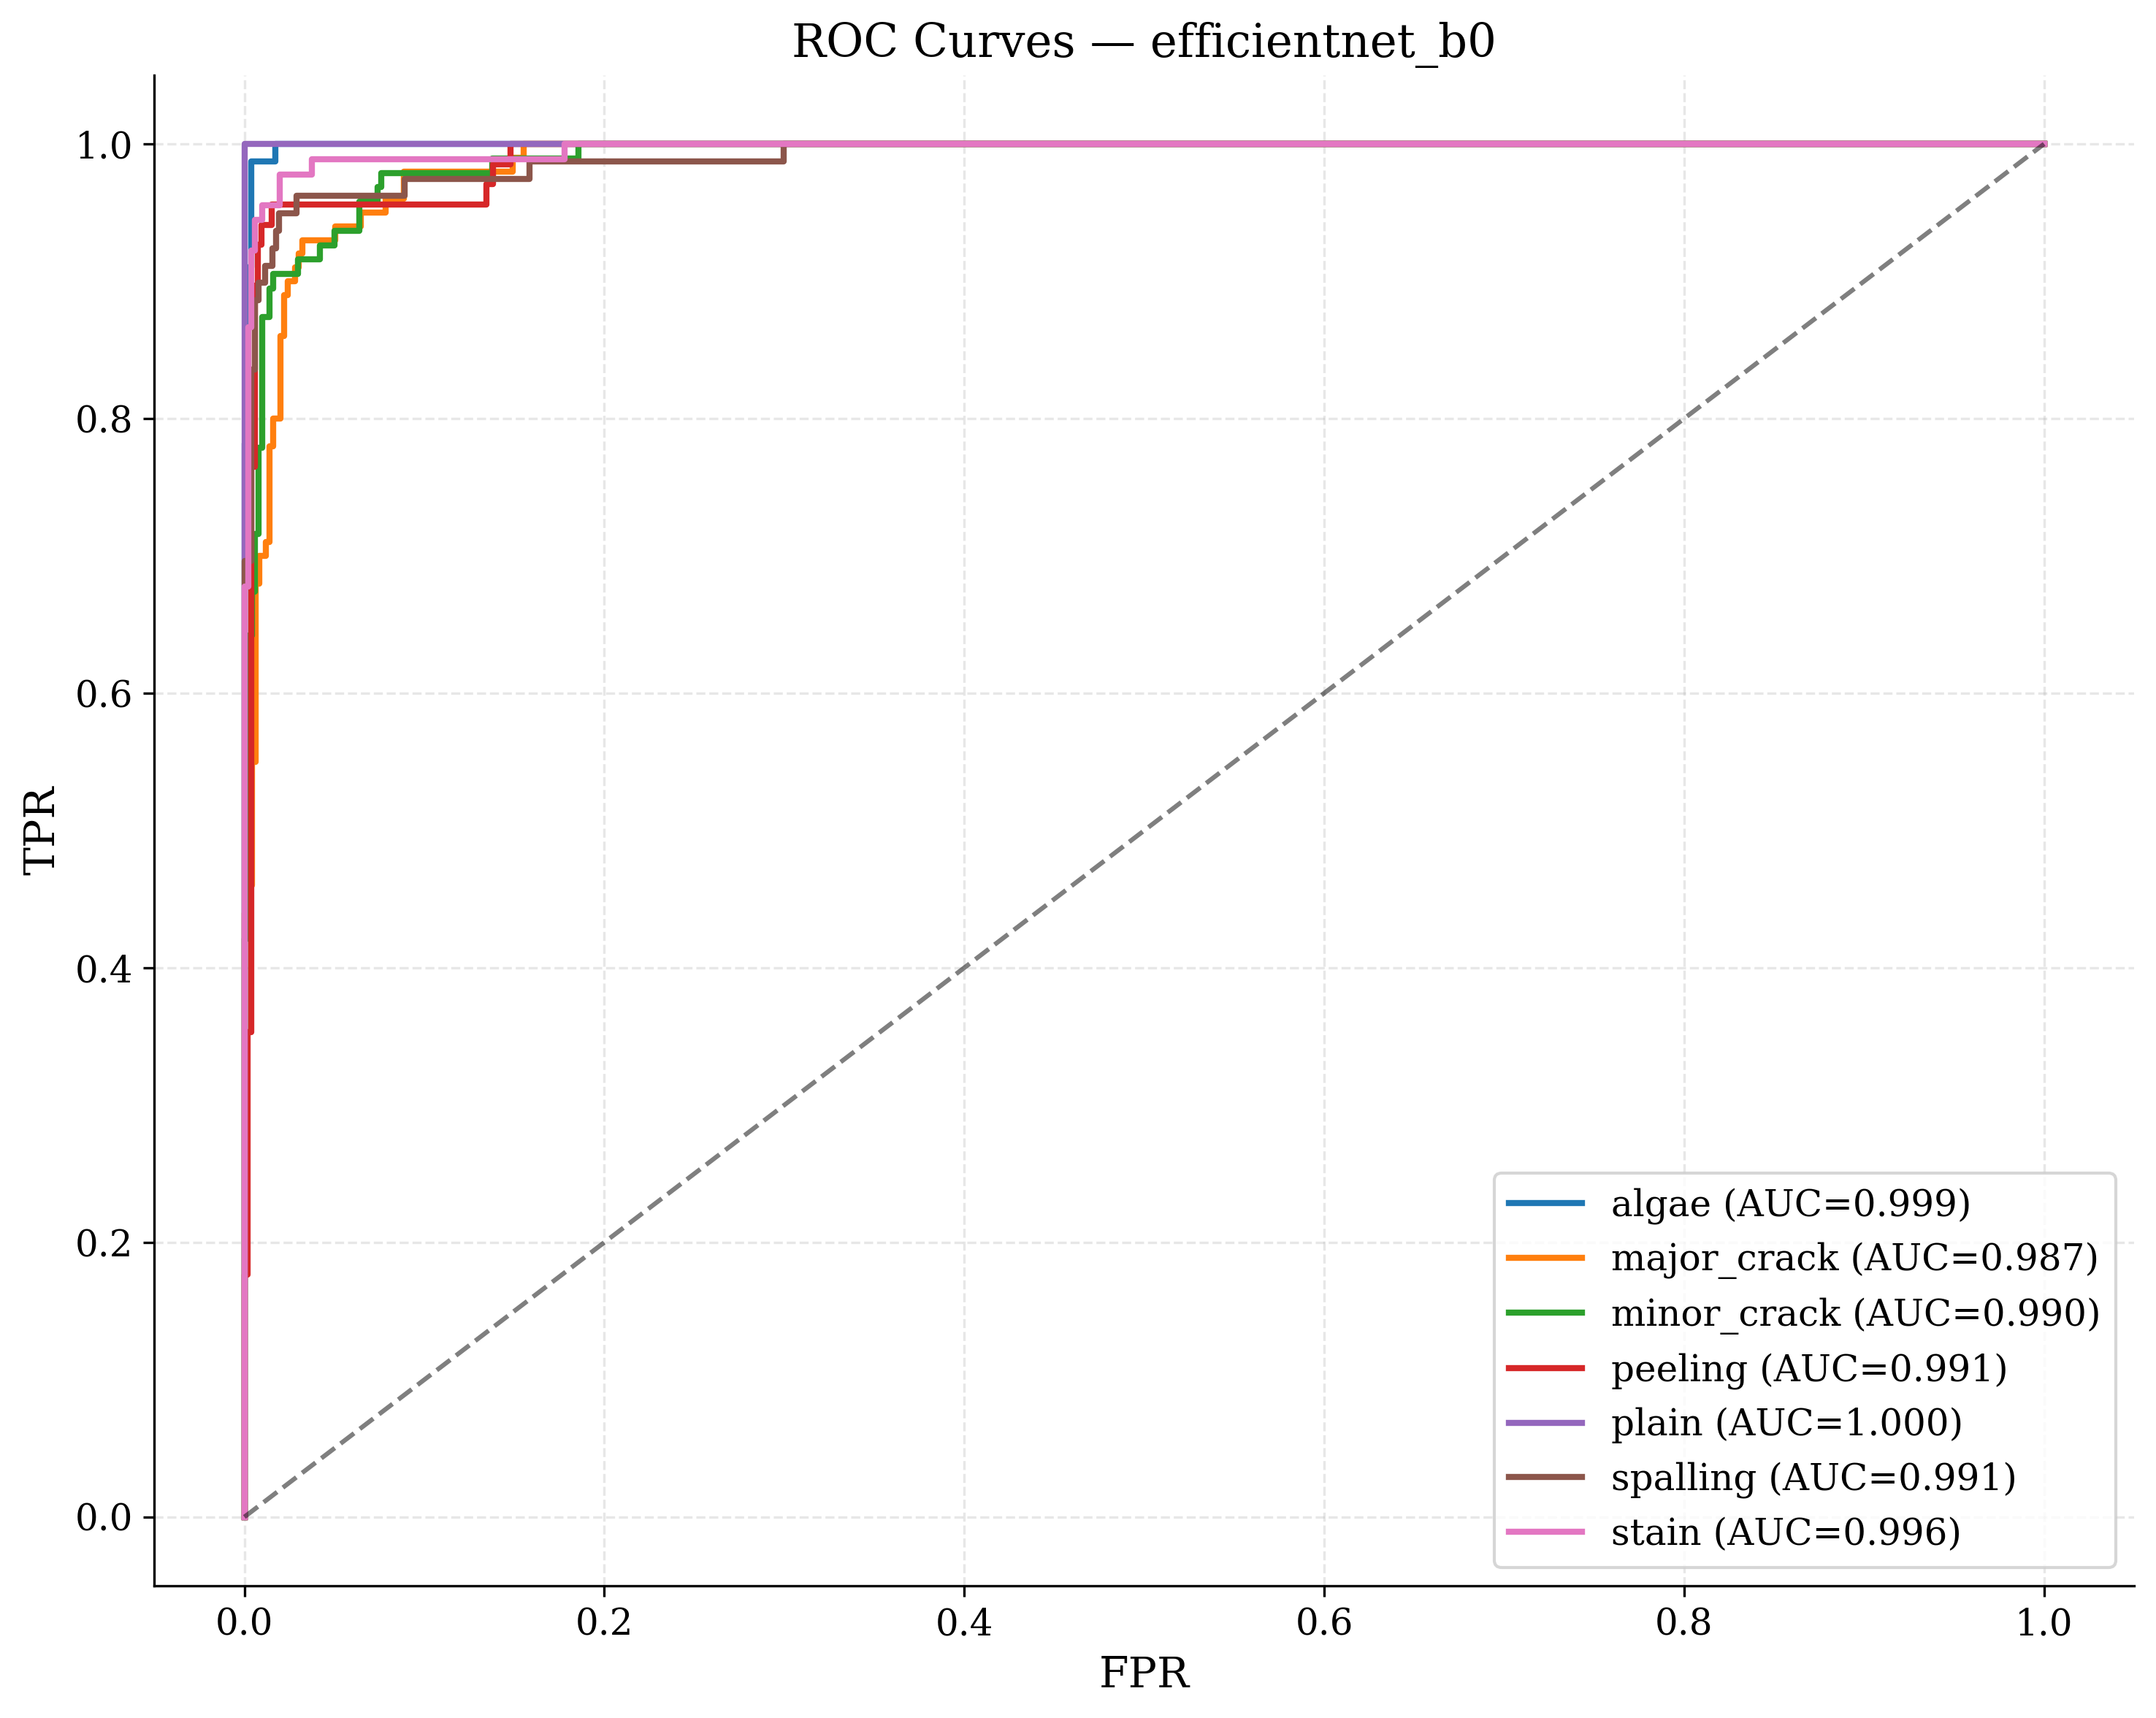
\includegraphics[width=\linewidth]{roc.png}}
\caption{ROC and Precision-Recall curves for EfficientNet-B0.}
\label{fig:roc_ap}
\end{figure}

\subsection{Per-Class F1-Score Heatmap}
Table~\ref{tab:f1_scores} shows F1-scores across models.

\begin{table}[htbp]
\caption{Per-Class F1-Scores (Models $\times$ Classes)}
\begin{center}
\begin{tabular}{|c|c|c|c|c|c|c|c|}
\hline
\textbf{Model} & algae & major\_crack & minor\_crack & peeling & plain & spalling & stain \\
\hline
EfficientNet-B0 & 0.981 & 0.887 & 0.904 & 0.916 & 0.994 & 0.914 & 0.955 \\
ResNet-18       & 0.950 & 0.886 & 0.911 & 0.914 & 0.989 & 0.928 & 0.913 \\
EfficientNet-V2-S & 0.949 & 0.851 & 0.893 & 0.879 & 0.989 & 0.889 & 0.954 \\
DenseNet-121    & 0.955 & 0.866 & 0.884 & 0.905 & 0.989 & 0.917 & 0.909 \\
MobileNet-V2    & 0.943 & 0.867 & 0.902 & 0.894 & 1.000 & 0.894 & 0.928 \\
\hline
\end{tabular}
\label{tab:f1_scores}
\end{center}
\end{table}

\begin{figure}[htbp]
\centerline{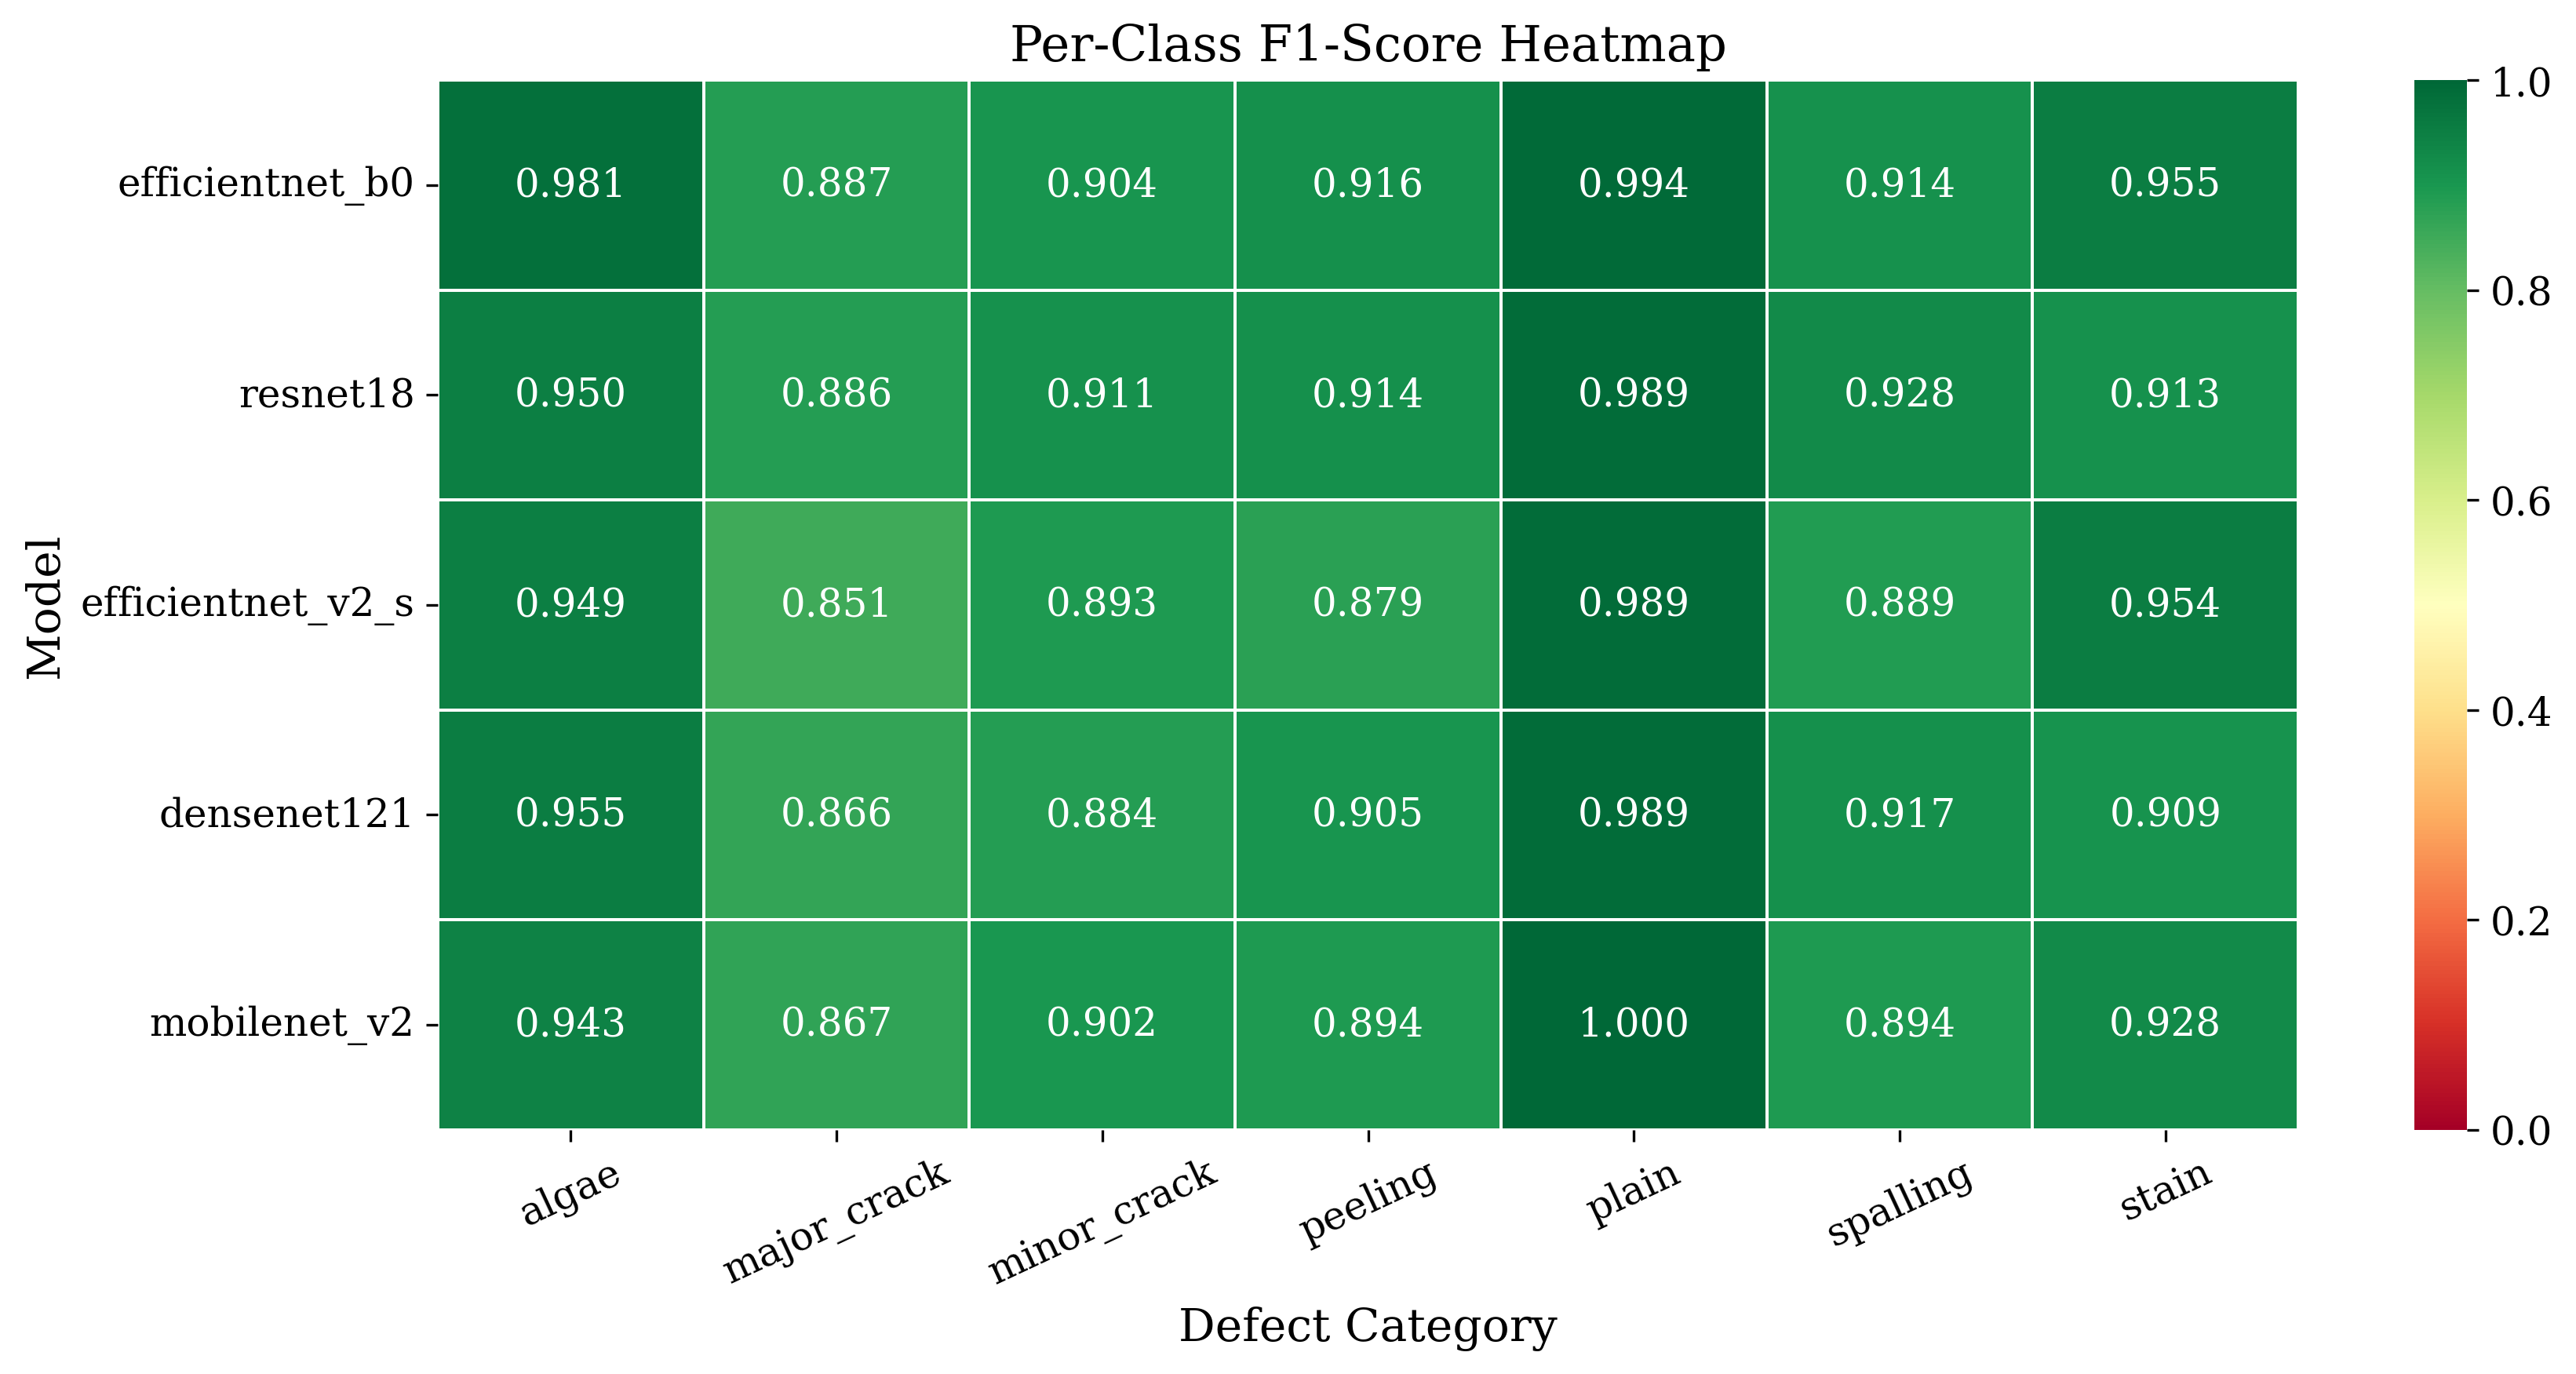
\includegraphics[width=\linewidth]{heatmap.png}}
\caption{F1-score heatmap for all models and defect classes.}
\label{fig:f1_heatmap}
\end{figure}




\clearpage




\section{Discussion}

\subsection{Performance Strengths and Model Efficacy}
The experimental results underscore the efficacy of transfer learning for structural defect detection in heritage buildings. Notably, all evaluated models exhibited rapid convergence, with EfficientNet-B0 achieving an 86.87\% validation accuracy within the initial epoch. This confirms that feature representations pretrained on the ImageNet dataset are highly transferable to the specific textural domains of historical masonry and structural materials. Furthermore, the implementation of a comprehensive data augmentation strategy---encompassing random flipping, rotation, color jittering, affine transformations, and random erasing---effectively mitigated overfitting. This is evidenced by the minimal generalization gap, with the difference between training and validation accuracies remaining strictly below 3--5\% at convergence across all architectures. In terms of overall system robustness, the proposed framework achieved a macro-average Area Under the Receiver Operating Characteristic Curve (AUC) of $\geq 0.993$ across all models. Such high discriminatory capability indicates a highly reliable ranking of defect probabilities, which is a critical prerequisite for automated triage in real-world structural inspection pipelines.

\subsection{Limitations and Algorithmic Challenges}
Despite the strong overall performance, several limitations and classification challenges were identified. The most prevalent misclassification occurred between the \textit{major crack} and \textit{minor crack} classes. This highlights an inherent ambiguity in severity classification, a morphological distinction that often necessitates specialized domain expertise to resolve, even for human annotators. Additionally, cross-class confusion was observed between \textit{peeling} and \textit{spalling} defects, resulting in approximately 6 to 9 misclassified samples per model. This error modality is primarily attributed to the frequent co-location of these defects on identical structural surfaces and their overlapping visual texture characteristics. 

A fundamental limitation of the current study is the scale of the dataset. Comprising 3,965 images, the corpus is relatively constrained for training deep neural networks from scratch or extensively fine-tuning high-capacity architectures. Consequently, future research will explore the integration of semi-supervised learning techniques and synthetic data generation frameworks, such as Generative Adversarial Networks (GANs), to systematically expand the training distribution. Finally, an architectural anomaly was noted regarding EfficientNet-V2-S. Despite possessing the highest parameter count (20.2 million), it yielded the lowest test accuracy among the evaluated models. This underperformance suggests that the current hyperparameter configuration---specifically the limited 30-epoch training budget and the fixed learning rate---is suboptimal for optimizing this larger model, indicating a need for targeted hyperparameter tuning in future iterations.


\section{Conclusion}

This study presented a comparative evaluation of five deep transfer learning architectures for the automated detection of surface defects in heritage structures. The experimental results demonstrate that ImageNet-pretrained models, when combined with aggressive data augmentation and reproducible training protocols, provide a robust and generalizable framework for structural health monitoring.

Among the evaluated architectures, EfficientNet-B0 emerged as the most efficient model, achieving a test accuracy of 93.46\% and a macro AUC of 0.994. With only 4.02 million parameters, this model offers an optimal balance between high classification performance and computational efficiency, making it particularly suitable for deployment on resource-constrained edge inspection devices.

Furthermore, the results confirm the effectiveness of transfer learning in this domain, as all five evaluated models achieved more than 91\% test accuracy and over 0.993 macro AUC. Class-wise performance analysis revealed that the \textit{plain} (no defect) and \textit{algae} categories are easily separable, while distinguishing between \textit{major crack} and \textit{minor crack} remains challenging due to their morphological similarities.




\begin{thebibliography}{00}

\bibitem{ref1}
H. S. Munawar, F. Ullah, A. Heravi, M. J. Thaheem, and A. Maqsoom, 
“Inspecting buildings using drones and computer vision: A machine learning approach to detect cracks and damages,” 
\textit{Drones}, vol. 6, no. 1, p. 5, Dec. 2021. doi: 10.3390/drones6010005.

\bibitem{ref2}
X. Zhou and R. L. K. Tiong, 
“Defects inspection system for building facades using drones and deep learning method,” 
\textit{Expert Systems with Applications}, vol. 298, Part B, p. 129715, Mar. 2026. 
doi: 10.1016/j.eswa.2025.129715.

\bibitem{ref3}
B. Ekanayake, 
“A deep learning-based building defects detection tool for sustainability monitoring,” 
in \textit{Proc. 10th World Construction Symposium (WCS)}, Y. G. Sandanayake, S. Gunatilake, and K. G. A. S. Waidyasekara, Eds., Sri Lanka, Jun. 2022, pp. 2–13. 
doi: 10.31705/WCS.2022.1.

\bibitem{ref4}
K. Chen, G. Reichard, X. Xu, and A. Akanmu, 
“Automated crack segmentation in close-range building façade inspection images using deep learning techniques,” 
\textit{Journal of Building Engineering}, vol. 43, p. 102913, Nov. 2021.

\bibitem{ref5}
Y. Liu, J. Yao, X. Lu, R. Xie, and L. Li, 
“DeepCrack: A deep hierarchical feature learning architecture for crack segmentation,” 
\textit{Neurocomputing}, vol. 338, pp. 139–153, Apr. 2019.

\bibitem{ref6}
G. Yang, K. Liu, J. Zhang, B. Zhao, Z. Zhao, and X. Chen, 
“Datasets and processing methods for boosting visual inspection of civil infrastructure: A comprehensive review and algorithm comparison for crack classification, segmentation, and detection,” 
\textit{Construction and Building Materials}, vol. 356, p. 129226, Nov. 2022.

\end{thebibliography}
\end{document}
